\documentclass[10pt,a4paper]{article}

\usepackage[a4paper,margin=25mm]{geometry}
\usepackage{amsmath}
\usepackage{enumitem}
\usepackage{graphicx}
\usepackage[most]{tcolorbox}
\usepackage{xcolor}
\usepackage{fancyhdr}
\usepackage{titlesec}
\usepackage{microtype}
\usepackage{hyperref}

\graphicspath{{../resources/}}

\definecolor{Terracotta}{HTML}{D97757}
\definecolor{Ink}{HTML}{1F1D1A}
\definecolor{SoftInk}{HTML}{5A554D}
\definecolor{Rule}{HTML}{DDD6C4}
\definecolor{Cream}{HTML}{FAF8F3}
\definecolor{Blue}{HTML}{3B6E8F}
\definecolor{Green}{HTML}{5A8A6A}
\definecolor{Gold}{HTML}{C9A961}

\hypersetup{colorlinks=true,linkcolor=Ink,urlcolor=Blue}
\pagestyle{fancy}
\fancyhf{}
\lhead{Lecture 1: Markets}
\rhead{An Economics of Everyday Institutions}
\cfoot{\thepage}
\renewcommand{\headrulewidth}{0.4pt}

\setlength{\parindent}{0pt}
\setlength{\parskip}{0.45em}
\setlist[itemize]{leftmargin=1.8em,itemsep=0.18em,topsep=0.25em}
\setlist[enumerate]{leftmargin=2em,itemsep=0.18em,topsep=0.25em}

\titleformat{\section}{\normalfont\Large\bfseries}{\thesection}{0.8em}{}
\titleformat{\subsection}{\normalfont\normalsize\bfseries}{\thesubsection}{0.8em}{}
\titlespacing*{\section}{0pt}{1.1em}{0.4em}
\titlespacing*{\subsection}{0pt}{0.8em}{0.25em}

\newtcolorbox{goalsbox}{
  enhanced,
  colback=white,
  colframe=Rule,
  boxrule=0.5pt,
  sharp corners,
  left=1.1em,
  right=1.1em,
  top=0.7em,
  bottom=0.8em,
  title=Learning goals,
  colbacktitle=SoftInk,
  coltitle=white,
  fonttitle=\bfseries,
  before upper={\setlength{\parskip}{0.35em}}
}

\newtcolorbox{keybox}[1]{
  enhanced,
  breakable,
  colback=Cream,
  colframe=Rule,
  boxrule=0.5pt,
  sharp corners,
  left=1em,
  right=1em,
  top=0.7em,
  bottom=0.7em,
  title=#1,
  colbacktitle=SoftInk,
  coltitle=white,
  fonttitle=\bfseries,
  before upper={\setlength{\parskip}{0.35em}}
}

\newtcolorbox{examplebox}[1]{
  enhanced,
  breakable,
  colback=Cream,
  colframe=Gold,
  boxrule=0.5pt,
  leftrule=2pt,
  sharp corners,
  left=1em,
  right=1em,
  top=0.7em,
  bottom=0.7em,
  title=Example: #1,
  colbacktitle=Gold,
  coltitle=white,
  fonttitle=\bfseries,
  before upper={\setlength{\parskip}{0.35em}}
}

\newtcolorbox{discussionbox}[1]{
  enhanced,
  breakable,
  colback=Cream,
  colframe=Terracotta,
  boxrule=0.5pt,
  leftrule=2pt,
  sharp corners,
  left=1em,
  right=1em,
  top=0.7em,
  bottom=0.7em,
  before skip=0.75em,
  after skip=0.75em,
  title=Discussion: #1,
  colbacktitle=Terracotta,
  coltitle=white,
  fonttitle=\bfseries\small,
  before upper={\setlength{\parskip}{0.35em}}
}

\newtcolorbox{conceptbox}[1]{
  enhanced,
  breakable,
  colback=Cream,
  colframe=Blue,
  boxrule=0.5pt,
  leftrule=2pt,
  sharp corners,
  left=1em,
  right=1em,
  top=0.7em,
  bottom=0.7em,
  title=Concept: #1,
  colbacktitle=Blue,
  coltitle=white,
  fonttitle=\bfseries\small,
  before upper={\setlength{\parskip}{0.35em}}
}

\newtcolorbox{insightbox}[1]{
  enhanced,
  breakable,
  colback=Cream,
  colframe=Green,
  boxrule=0.5pt,
  leftrule=2pt,
  sharp corners,
  left=1em,
  right=1em,
  top=0.7em,
  bottom=0.7em,
  title=Takeaway: #1,
  colbacktitle=Green,
  coltitle=white,
  fonttitle=\bfseries,
  before upper={\setlength{\parskip}{0.35em}}
}

\newtcolorbox{quotebox}[2]{
  enhanced,
  breakable,
  colback=white,
  colframe=Rule,
  boxrule=0.45pt,
  leftrule=2.5pt,
  sharp corners,
  left=1.1em,
  right=1.1em,
  top=0.75em,
  bottom=0.7em,
  before skip=0.75em,
  after skip=0.75em,
  title=#1,
  colbacktitle=Cream,
  coltitle=Ink,
  fonttitle=\bfseries\small,
  after upper={\par\smallskip\hfill{\normalfont\footnotesize\color{SoftInk}#2}},
}

\title{\vspace{-2em}\bfseries Lecture 1: Markets, and Where They Stop}
\author{An Economics of Everyday Institutions}
\date{Day 1}

\begin{document}
\maketitle
\thispagestyle{fancy}

\begin{goalsbox}
\begin{itemize}
  \item See markets as institutions, not as the natural background of social life.
  \item Ask why markets appear in some places but not in others.
  \item Separate three questions: what a market does, how it came to be, and whether it should exist.
  \item Set up later lectures on externalities, asymmetric information, incomplete contracts, and non-market institutions.
\end{itemize}
\end{goalsbox}

\begin{keybox}{The plan}
This lecture is not a full theory of markets. It is an opening problem. We start with familiar and strange examples of exchange, then ask why some things become market goods while others do not.

The important habit is to avoid treating ``market'' as a yes-or-no moral slogan. A market may be useful because it coordinates information and incentives. It may fail because important costs are missing from the price. It may be blocked because quality is hard to observe. It may be rejected because pricing the thing changes what the thing means.
\end{keybox}

\section{Same Money, Different Reaction}

\begin{examplebox}{School}
Case A: Before an exam, you buy a test-prep book for 80 yuan. Nobody finds this unusual.

Case B: After the exam, you offer 500 yuan to the top student in class and ask them to transfer their rank to you. Suppose they agree.
\end{examplebox}

\begin{examplebox}{Time}
Case A: During evening study, you pay 15 yuan for food delivery. A rider spends 20 minutes bringing food to you. Someone's time has been priced, but the transaction feels ordinary.

Case B: On your eighteenth birthday, you pay a stranger 300 yuan to spend the evening with you. Again, someone's time has been priced. This feels different.
\end{examplebox}

\begin{discussionbox}{First reactions}
What exactly changes between the two cases? Is the problem consent, money, the type of good, third-party effects, or the meaning of the relationship?
\end{discussionbox}

These examples are useful because they make a simple point: a market is not just ``voluntary exchange with money.'' Even when both sides agree, we may still ask whether the object is tradable, whether the transaction affects other people, and whether pricing the thing changes its social meaning.

\section{Markets Around Us}

Start with easy cases: vegetable markets, housing markets, stock markets, second-hand textbook markets, tutoring markets, and online resale markets.

Then add cases that are less obvious: scalped concert tickets, paid queueing, leaked exam papers, domain names, celebrity greeting videos, prediction markets.

\begin{figure}[h]
\centering
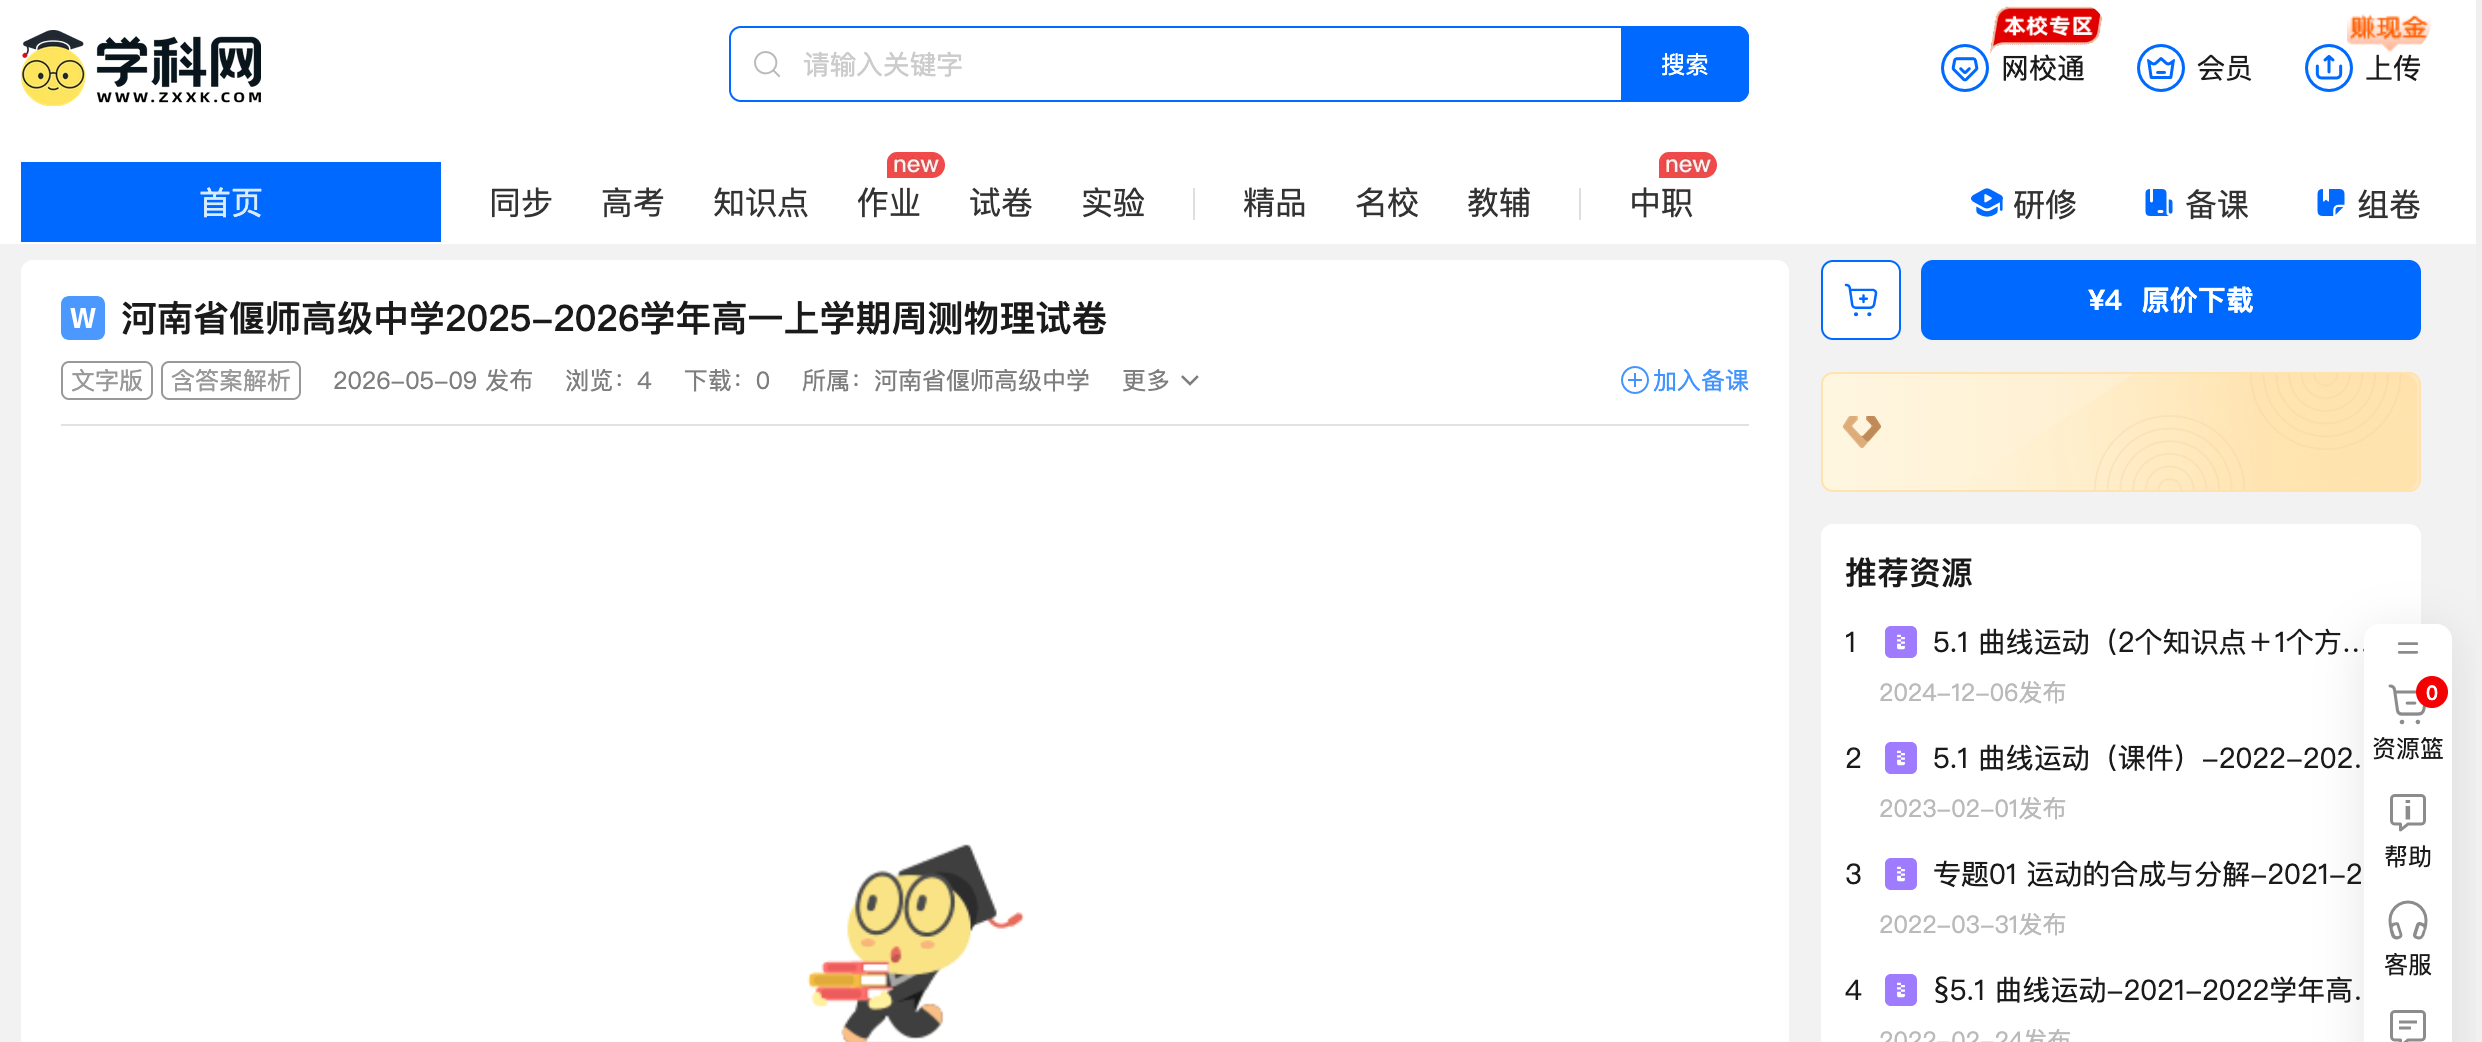
\includegraphics[width=0.68\linewidth]{shijuan.png}
\caption{Even test papers and practice materials can become market goods.}
\end{figure}

\begin{discussionbox}{Minimum conditions}
If there is a buyer, a seller, and a price, is that already enough to call something a market? What else is needed?
\end{discussionbox}

\section{Stranger Markets}

\subsection{Domain Names}

A domain name is not a physical object. It is a position in an address system. Yet it can be scarce, owned, transferred, and priced. People register names cheaply and later resell them at much higher prices.

The \texttt{.ai} domain is a good example. It originally belongs to Anguilla, a small British overseas territory. The AI boom turned this country-code domain into a valuable asset. The exact revenue numbers change from year to year, so they should be checked before class, but the example is clear: a technical naming convention can become a market asset.

\subsection{Celebrity Greeting Videos}

On platforms such as Cameo, users pay celebrities or internet personalities to record short personalized videos. The file itself is not the main point. What is being bought is attention, recognition, and the feeling that a particular person spent a few seconds addressing you.

\subsection{Prediction Markets}

Prediction markets allow people to buy and sell contracts tied to future events. If a contract pays one dollar when an event happens, its price can be read as a rough market-implied probability.

\begin{examplebox}{A strange contract}
A prediction market can even create a contract on an extreme or absurd event. The point is not whether the event is likely. The point is that a future contingency can be written into a tradable contract.

\begin{center}
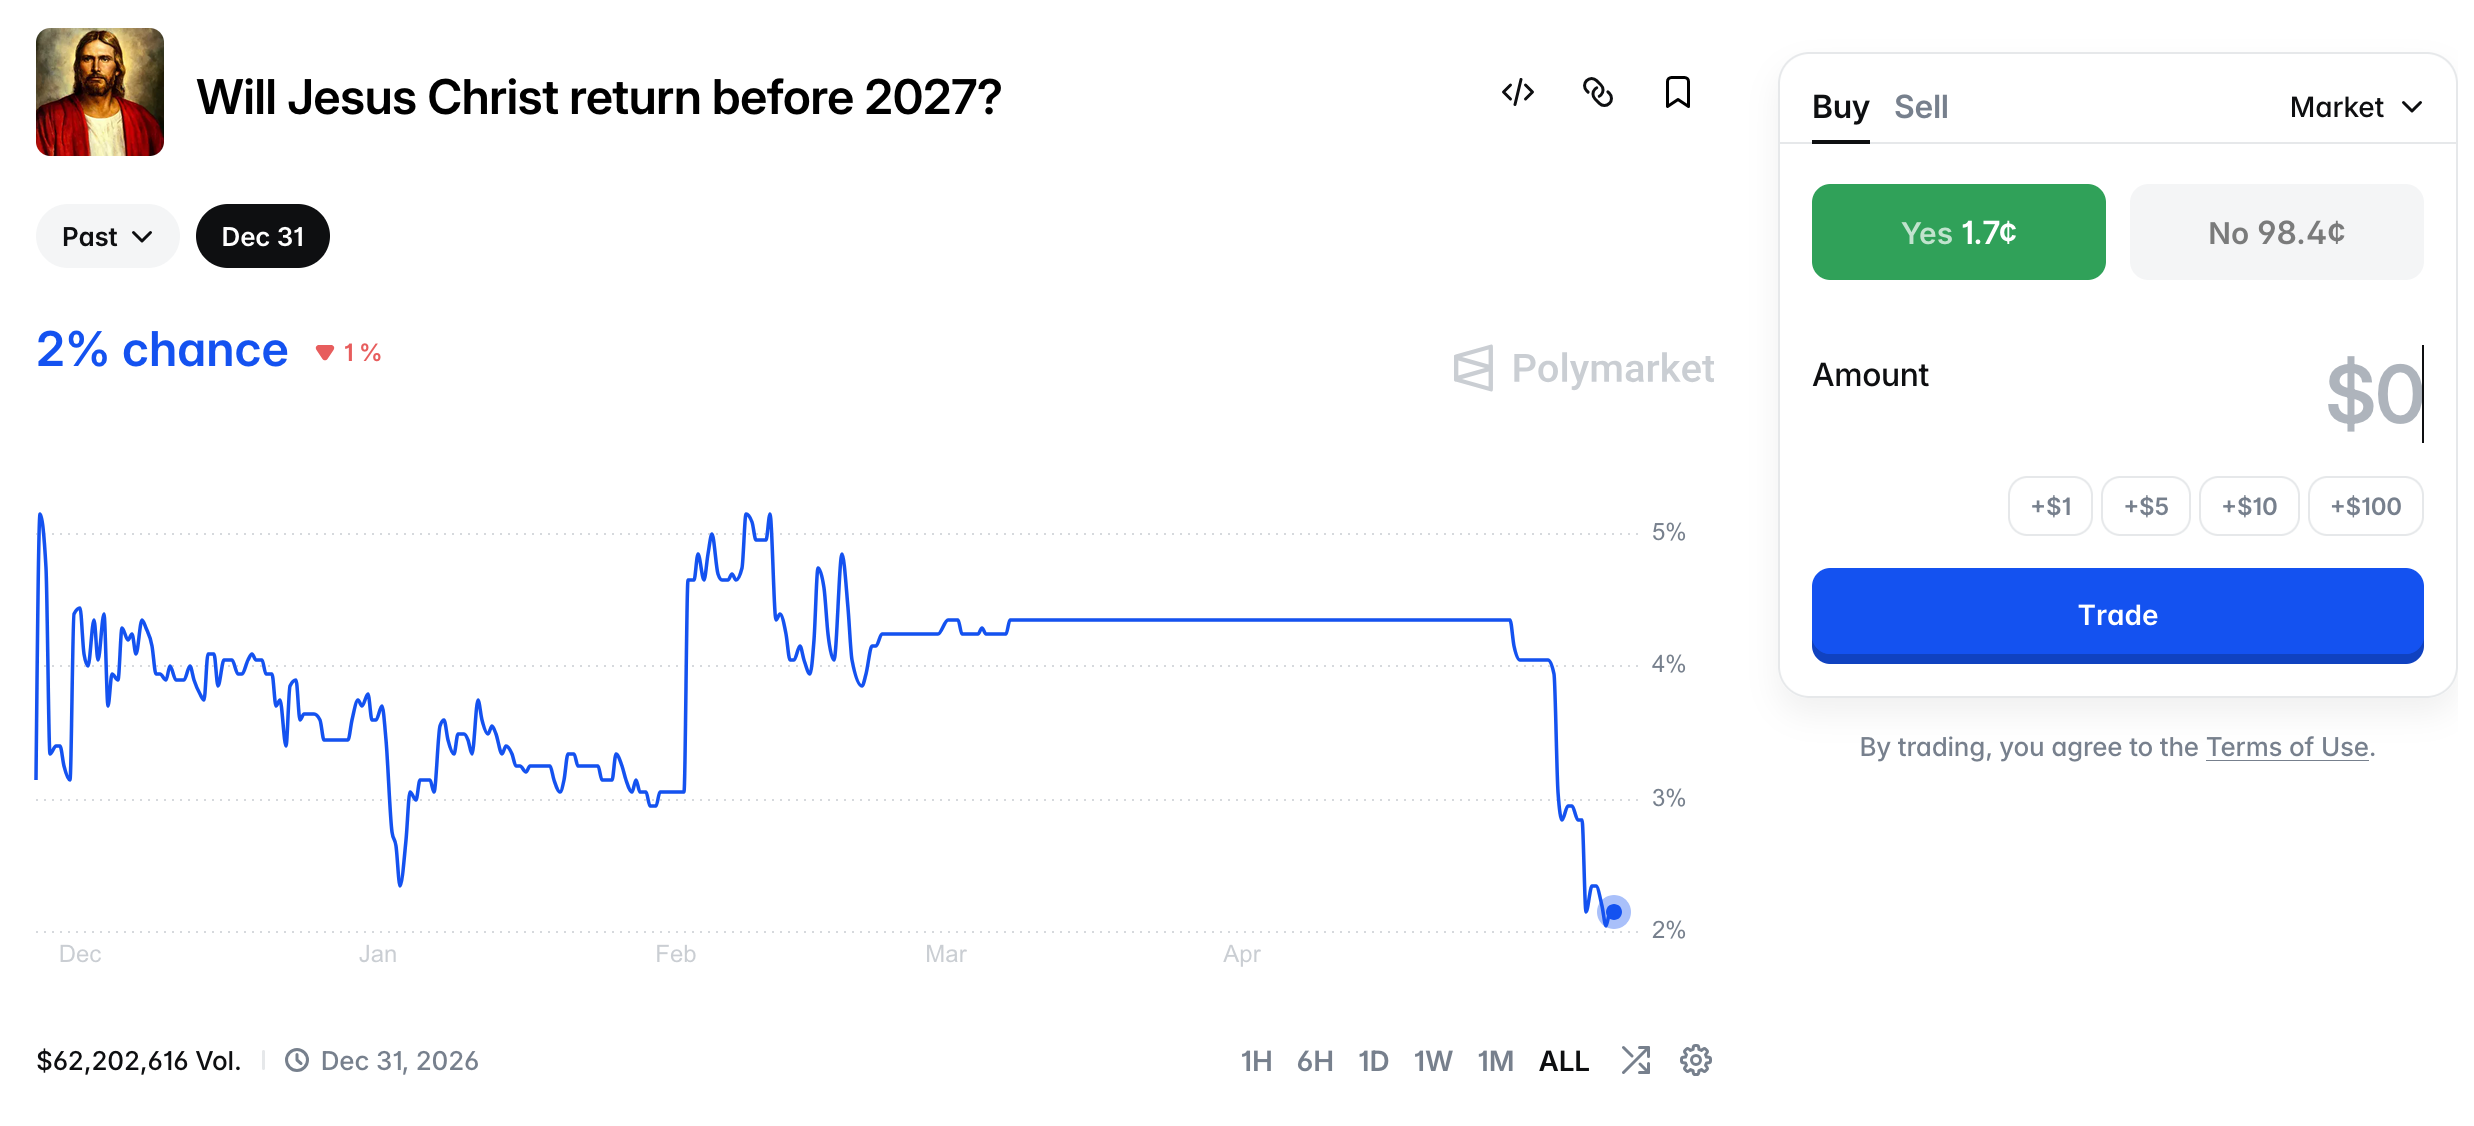
\includegraphics[width=0.72\linewidth]{polymarket.png}
\end{center}
\end{examplebox}

\begin{discussionbox}{Prediction or gambling?}
Why create such markets? Are they aggregating information, helping people hedge risk, or simply creating a new form of gambling?
\end{discussionbox}

\section{Markets That Do Not Exist}

Now reverse the question. If so many things can be traded, what cannot be traded?

Exam ranks usually cannot be sold. Friendship cannot simply be bought. Votes are not supposed to be sold. Mathematical formulas are normally free to use:
\[
x = \frac{-b \pm \sqrt{b^2 - 4ac}}{2a}.
\]

But songs can be copyrighted, patents can be licensed, and software can be sold. So the issue is not simply ``knowledge should be free'' or ``knowledge should be owned.'' Different kinds of knowledge fit different institutional arrangements.

The quadratic formula is non-rival: your use does not prevent my use. Charging every user would create large access costs and slow down later learning and invention. Basic science is often rewarded through reputation, priority, jobs, grants, prizes, and public funding rather than through a fee on every act of use.

\begin{insightbox}{Markets are not the only incentive system}
Prices and property rights are one way to create incentives. They are not the only way. Sometimes strong exclusion helps production. Sometimes it blocks use and follow-on creation.
\end{insightbox}

\section{When Can a Market Exist?}

A market usually needs several conditions:

\begin{enumerate}
  \item \textbf{Scarcity.} If a thing is not scarce, pricing it is usually unnecessary.
  \item \textbf{Tradability.} The thing must be separable enough to be transferred or controlled.
  \item \textbf{Gains from trade.} Buyers and sellers need a reason to exchange.
  \item \textbf{Participants.} There must be enough buyers, sellers, or at least enough recognized value.
  \item \textbf{Price formation.} Prices may come from bargaining, auctions, posted prices, or competition.
  \item \textbf{Institutional support.} Property rights, contract enforcement, ratings, disclosure rules, and dispute resolution reduce the cost of trading.
  \item \textbf{Technology.} Search, matching, monitoring, and payment technologies can make previously difficult markets possible.
\end{enumerate}

\begin{insightbox}{Why markets appear}
One efficiency reason for markets is that prices compress dispersed information. A person does not need to know every cause of a shortage. A price change is enough to change behavior.

But this explanation has limits. A missing market may reflect high transaction costs, unclear property rights, hard-to-observe quality, external costs, moral rejection, or historical accident. So the question is not only whether a market would be efficient. It is also what has to be built, protected, or accepted before the market can work.
\end{insightbox}

\section{If Not Markets, Then What?}

Scarce resources can be allocated in many ways:

\begin{itemize}
  \item \textbf{Queueing:} first come, first served. The cost is time.
  \item \textbf{Lottery:} random allocation. It may be equal, but it ignores intensity of need.
  \item \textbf{Administrative criteria:} allocation by need, urgency, income, score, or status.
  \item \textbf{Power and connections:} informal but common.
  \item \textbf{Exams and competitions:} allocation by performance, though performance itself may depend on family resources.
\end{itemize}

None of these mechanisms is clean. Queueing favors those with time. Markets favor those with money. Administrative rules can be gamed. Exams may look meritocratic while importing inequality from elsewhere.

\begin{insightbox}{Markets may reappear}
Choosing a non-market allocation rule does not make scarcity disappear. Train tickets allocated by queueing may produce scalpers. Hospital registration may produce ticket brokers. Free university visit slots may be resold. When scarcity remains, market forces often return through the side door.
\end{insightbox}

\section{How Do Markets Come About?}

\begin{keybox}{The puzzle}
Markets are strange objects. They involve many people who do not know one another, often do not care about one another, and usually do not understand the whole system they are part of. Still, some order appears: food arrives in shops, domain names acquire prices, tickets are resold, workers are hired, and futures are traded.

The question is not only whether markets are good or bad. The first question is simpler and harder: how can this kind of order come about at all?
\end{keybox}

\subsection{Some Powerful Answers}

Smith is writing about a commercial society in which each person depends on the cooperation of many strangers. I cannot make my own bread, clothes, books, phone, and transport. Nor can I rely on everyone else's kindness. The ordinary solution is exchange: I get what I need by offering others something they have reason to accept.

\begin{quotebox}{Adam Smith}{The Wealth of Nations, 1776}
``It is not from the benevolence of the butcher, the brewer, or the baker, that we expect our dinner, but from their regard to their own interest.''
\end{quotebox}

The reasoning has three steps. First, begin with individuals rather than with ``society'' as a single actor. Second, look at what each person can offer and what each person wants. Third, ask how many such local exchanges can add up to a larger order: bread gets baked, shops are stocked, and people who never planned together still become connected through prices and trade.

Mandeville gives a deliberately more disturbing version of this thought. \textit{The Fable of the Bees} imagines a prosperous hive driven by vanity, luxury, pride, and competition. Its point is not a simple moral lesson. It is a provocation against the idea that public order must come from private virtue.

\begin{quotebox}{Bernard Mandeville}{The Fable of the Bees, 1714}
``Thus every Part was full of Vice, Yet the whole Mass a Paradice; ... Their Crimes conspired to make 'em Great.''
\end{quotebox}

Smith gives the cleaner analytical version; Mandeville gives the unsettling version. Together they introduce the tradition of unintended order. The point is not that people are selfish in every situation, or that selfishness is good. The point is that social order may arise from many separate actions without anyone intending the final pattern. This removes a tempting assumption: if something is orderly, someone must have designed it.

\begin{quotebox}{F. A. Hayek}{The Counter-Revolution of Science, 1952}
``some sort of order arises as a result of individual action but without being designed by any individual''
\end{quotebox}

Hayek makes the methodological point explicit. If an outcome is directly designed, we can study the designer's intention. If it is a natural event, we can study nature. But many social outcomes are neither: no single person intends a traffic jam, a tutoring arms race, a scalping market, or a price pattern. These outcomes are produced by actions, but not chosen as a whole. That is why they need social-scientific explanation.

Weber asks a different question. He is not mainly asking how scattered exchanges can coordinate. He is asking what makes modern capitalism distinctive. His answer emphasizes rational calculation. Large-scale market activity requires more than desire to trade: actors must be able to calculate costs, revenues, debts, risks, and future obligations in a relatively stable environment.

\begin{quotebox}{Max Weber}{General Economic History, 1923}
``a rational capitalistic establishment is one with capital accounting ... which determines its income yielding power by calculation''
\end{quotebox}

This is powerful for the opposite reason. It stops us from imagining markets as pure spontaneity. People can make contracts, invest, lend, hire, and trade at scale only when rules are reasonably predictable: property can be recorded, contracts can be enforced, money can be counted, firms can keep accounts, and officials apply rules in a relatively regular way. The market depends on a great deal of non-market infrastructure.

Marx begins from another angle. He does not begin with exchange as a solution to coordination, or with calculation as a condition of modern markets. He begins with the commodity, because capitalist society appears to us as a world in which more and more things are produced for sale.

\begin{quotebox}{Karl Marx}{Capital, Volume I, 1867}
``The wealth of societies in which the capitalist mode of production prevails, appears as a gigantic collection of commodities''
\end{quotebox}

Marx pushes the question further into history: how did labor, land, and other conditions of life become commodities in the first place? That question matters because it reminds us that markets are not just mechanisms. They are historical arrangements. Things become buyable and sellable through social change, conflict, law, and power.

\begin{insightbox}{Why these answers matter}
Smith and Mandeville help us see emergent order. Hayek names the aggregation problem: individual actions can produce outcomes no one designed. Weber helps us see calculable order. Marx helps us see historical transformation. Each answer makes markets thinkable, but each also leaves something out. A spontaneous-order story can make markets look too natural. A Weberian story can make modern order look too clean. A Marxian story can make market society look too dominated by conflict.
\end{insightbox}

\subsection{The Mission of This Course}

This course starts from everyday institutions: markets, queues, property rights, contracts, firms, families, platforms, and rules that seem too ordinary to notice. The goal is not to memorize one grand theory of society. The goal is to learn how to ask better questions about arrangements that usually sit in the background of daily life.

We will return to three questions:

\begin{enumerate}
  \item How did this arrangement become possible?
  \item What problem does it solve, and through what incentives or constraints?
  \item What does it leave out, distort, or make worse?
\end{enumerate}

Economics is especially useful for the second question. It turns a complicated social object into something thinkable by simplifying it in a disciplined way.

\subsection{The First Tool: Economic Thinking}

For any institution or market-like arrangement, start with six questions:

\begin{conceptbox}{Economic thinking}
\begin{itemize}
  \item \textbf{Players:} Who is involved? Avoid saying ``society wants'' or ``the school wants'' too quickly. Large groups usually contain smaller actors with different incentives.
  \item \textbf{Actions and constraints:} What can each player actually do, and what rules make those actions possible or impossible?
  \item \textbf{Incentives:} What does each player care about? Money, time, grades, reputation, risk, convenience, fairness?
  \item \textbf{Information:} What does each player know, and what do they not know?
  \item \textbf{Aggregation:} How do individual choices add up to a larger outcome?
  \item \textbf{Equilibrium:} Given the rules and what others are doing, does any player have a reason to change their behavior?
\end{itemize}
\end{conceptbox}

Take paid queueing as an example. The players are not just ``buyers'' and ``sellers.'' There are people waiting in line, people with less time, people with less money, the organizer of the queue, and sometimes professional queue-sellers. The actions include waiting, paying, reselling, blocking resale, or changing the rule. The incentives differ: some people want to save time, some want income, some want the queue to look fair.

The Smith-style question is: why would this trade appear if no one designed a formal market for queue positions? The Weber-style question is: under what rules can a queue position become transferable at all? The economic move is to list the players, actions, incentives, information, and rules, then ask how their choices aggregate into a stable pattern.

\section{What Do Markets Do Well?}

Markets often work because they combine information and incentives.

\begin{itemize}
  \item Prices signal relative scarcity.
  \item Profit and loss give people reasons to respond.
  \item Specialization allows people to produce what they are comparatively good at.
  \item Competition pressures sellers to pay attention to buyers.
\end{itemize}

This is the same logic introduced earlier: ordinary coordination can emerge from people responding to their own situations, even when no one is trying to coordinate the whole system.

\section{Where Do Markets Go Wrong?}

The same mechanism can also create problems.

\begin{itemize}
  \item \textbf{Ability to pay is not the same as need.} School-district housing, masks, and concert tickets may go to those who can pay most, not those who need most.
  \item \textbf{Some costs fall on outsiders.} Pollution, traffic, noise, and platform labor pressure may affect people outside the transaction.
  \item \textbf{Quality may be hard to observe.} Medical services, used cars, tutoring, and financial products are difficult for buyers to judge.
  \item \textbf{Pricing may change meaning.} Friendship, public honors, votes, and academic ranks are not just scarce objects. They are embedded in social meanings.
\end{itemize}

\begin{discussionbox}{Evaluation}
Pick one case: masks during a shortage, school-district housing, ticket scalping, medical services, food delivery platforms, or paid queueing. What problem does the market solve? What problem does it create?
\end{discussionbox}

\section{Three Different Questions}

The phrase ``market boundary'' hides several different questions.

\begin{enumerate}
  \item \textbf{Functional question:} What does this boundary do? Does it reduce transaction costs, protect third parties, solve information problems, or preserve incentives?
  \item \textbf{Historical question:} Why did the boundary end up here rather than somewhere else?
  \item \textbf{Normative question:} Should this thing be for sale?
\end{enumerate}

Economics is strongest on the first question. It can also say something about the second, especially when different stable arrangements are possible. It has no special authority over the third. Efficiency arguments can inform moral judgment, but they do not replace it.

\begin{insightbox}{A common mistake}
People often slide between the three questions. ``This market is inefficient'' may secretly mean ``I find it morally wrong.'' ``This market exists'' may be mistaken for ``this market is justified.'' Keep the questions separate.
\end{insightbox}

\section{Questions for Later}

This lecture leaves several questions open:

\begin{itemize}
  \item If a transaction affects outsiders, can the price still reflect the real cost? This leads to externalities.
  \item If one side knows much more than the other, can market exchange still work well? This leads to asymmetric information.
  \item If contracts cannot specify everything, why do firms and other organizations exist? This leads to incomplete contracts and firm boundaries.
  \item If a non-market institution seems functional but also unequal or oppressive, how should we explain it without justifying it? This leads to the final comparative discussion.
\end{itemize}

\begin{insightbox}{Closing point}
A market is not a natural background. It is an institutional arrangement. We need to explain why it appears, why it stops, and what follows from using it.
\end{insightbox}

\end{document}
